\graphicspath{{content/3_results/figures}}

\section{Voltage Regulation}

\subsection{Measured}

As mentioned in the design section, feedback resistors need to be chosen. According to \cite{datasheetLD1117}, $R_2$ in Figure \ref{fig:voltageRegulation_5v}
can be calculated using $V_{out} = V_{ref} (1 + \frac{R2}{R1})$. With $V_{out} = \SI{5}{V}$, $V_{ref} \approx \SI{1.25}{V}$, and $R_1 = \SI{120}{\ohm}$,
$R_2 = R_1 \cdot \left(\frac{V_{out}}{V_{ref}} - 1\right) = \SI{360}{\ohm}$. A $\SI{470}{\ohm}$ potentiometer was used for the practical circuit to adjust the output to exactly $\SI{5}{V}$.

\begin{figure}[!htb]
    \centering
    \begin{minipage}{.45\textwidth}
        \centering
        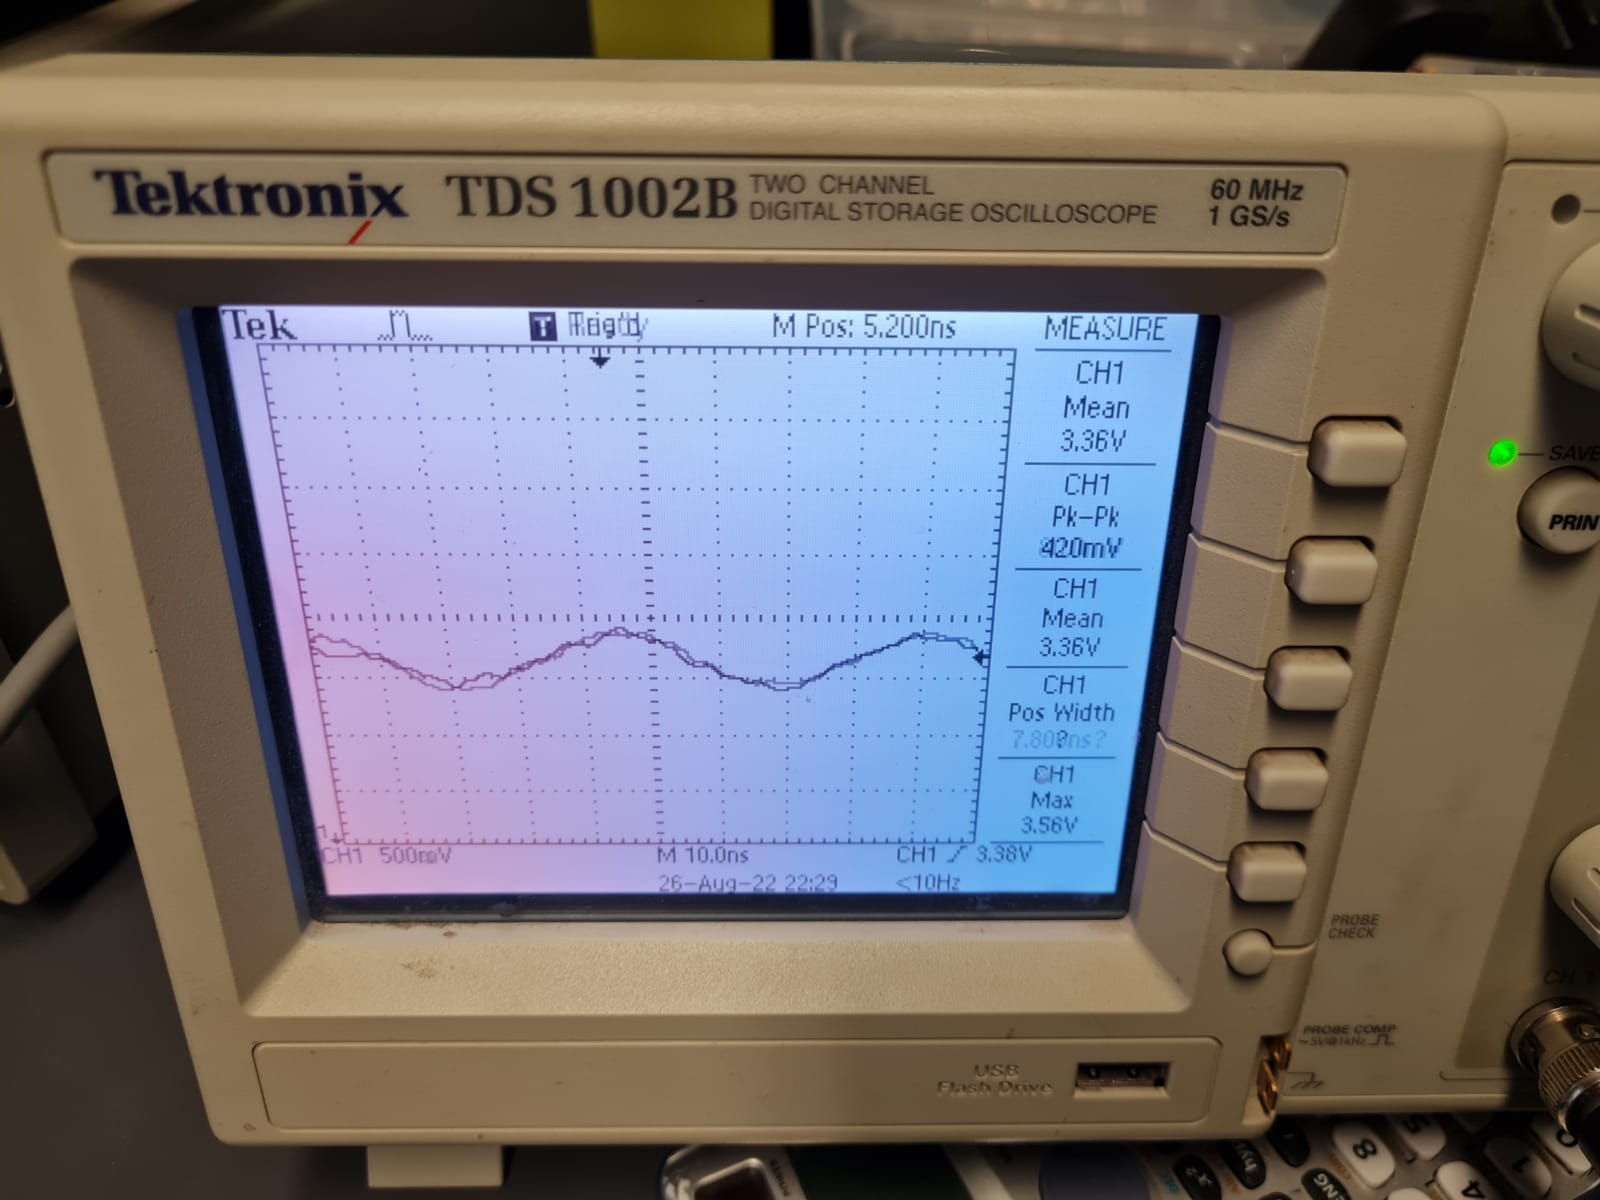
\includegraphics[width=1.0\linewidth]{voltageRegulation_3v3}
        \captionof{figure}{3.3 V Regulator Ripple Measurement}
        \label{fig:voltageRegulation_measure_3v3}
    \end{minipage}
    \begin{minipage}{.45\textwidth}
        \centering
        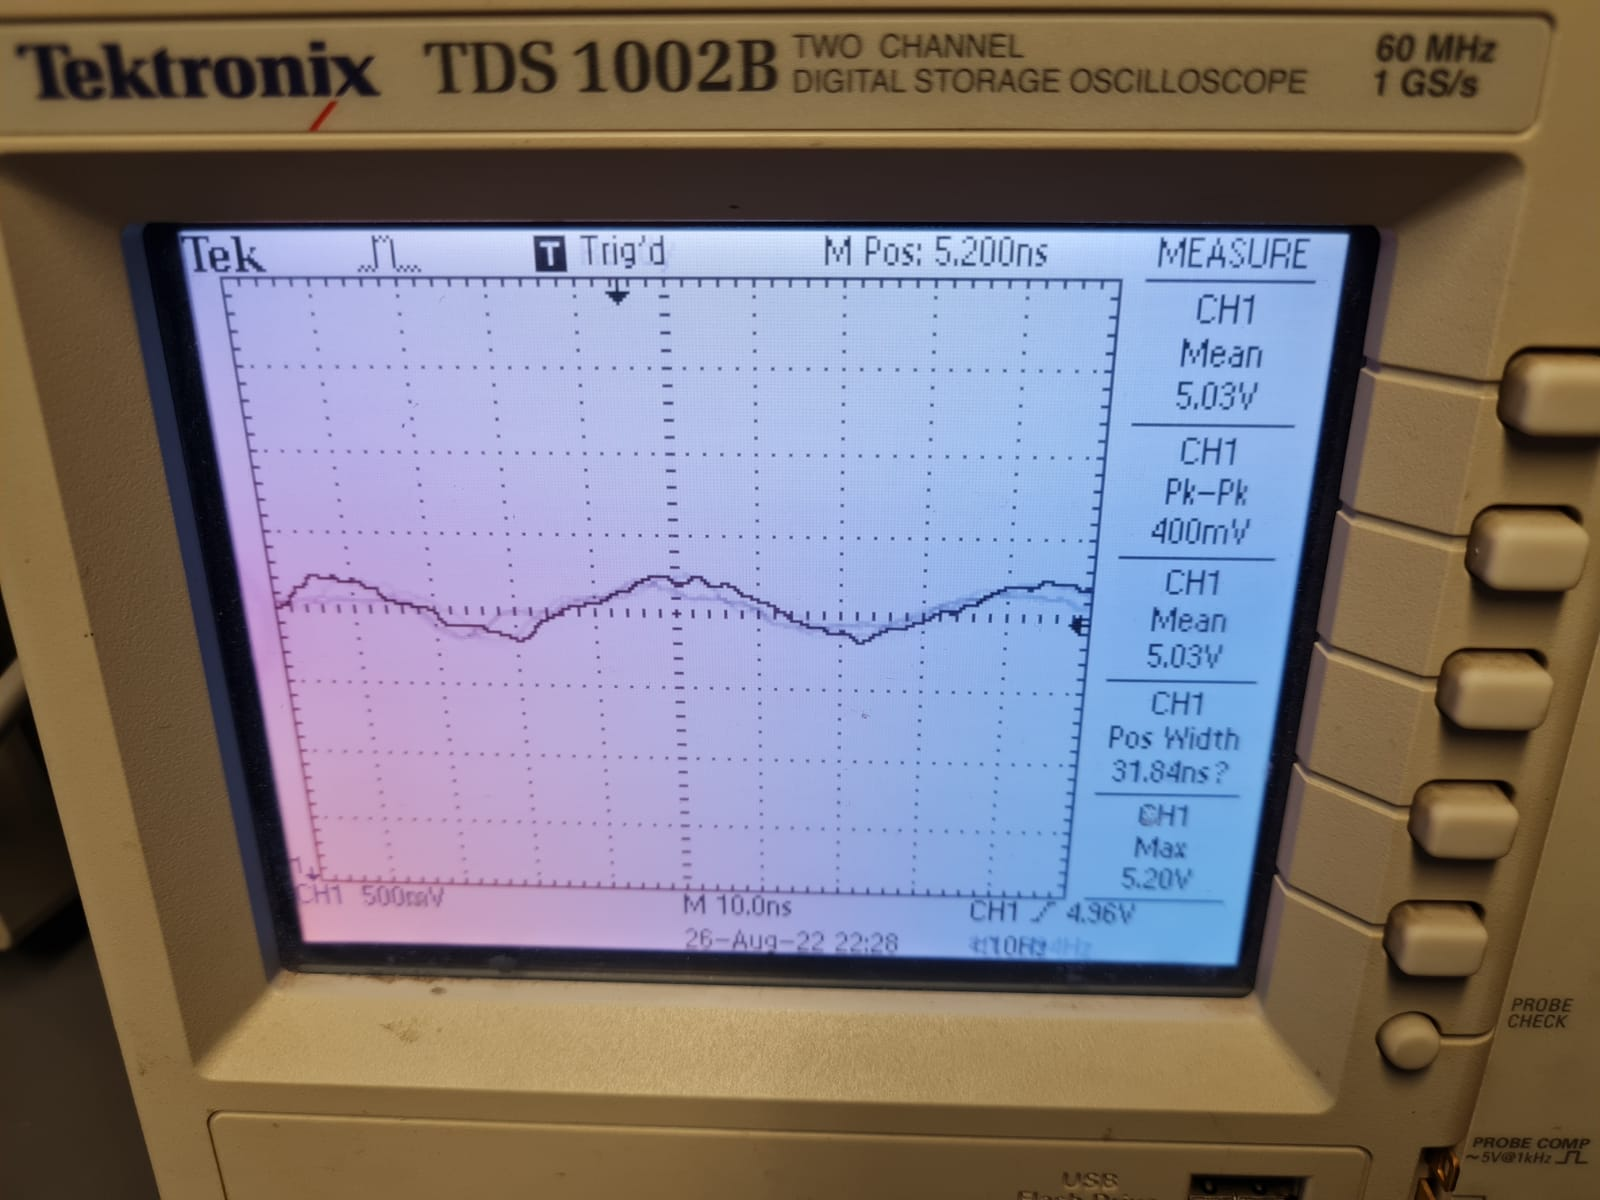
\includegraphics[width=1.0\linewidth]{voltageRegulation_5v}
        \captionof{figure}{5 V Regulator Ripple Measurement}
        \label{fig:voltageRegulation_measure_5v}
    \end{minipage}
\end{figure}

The ripple in the above figures was measured under full motor load with the worst-case results being shown. Although these results
are rather large ($\approx \SI{200}{mV}$ deviation from the regulated value), the nominal deviation was less than $\SI{50}{mV}$.